\section{Inter-Integrated Circuit Protocol}

Inter-Integrated Circuit (I2C), like SPI,
is a serial communication protocol.
Designed for low-cost, medium data rate applications,
I2C is the de facto standard for 2-wire communications.
I2C is serial, byte-oriented, multi-master,
and multi-slave. It has a serial data line
(SDA) and serial clock line (SCL), which
need to be pulled up with resistors.
It supports up to 100 kilobits a second
in standard mode and 400 kilobits a second
in fast mode.

SDA and SCL must be open-drain, connected
to positive if the output is 1 and in
high impedance state if the output is 0.
The internal pull-up resistor is too weak,
so we require external pull-up resistors
on SDA and SCL (2k$\Omega$ for fast mode and
10k$\Omega$ for standard mode).

\begin{figure}
    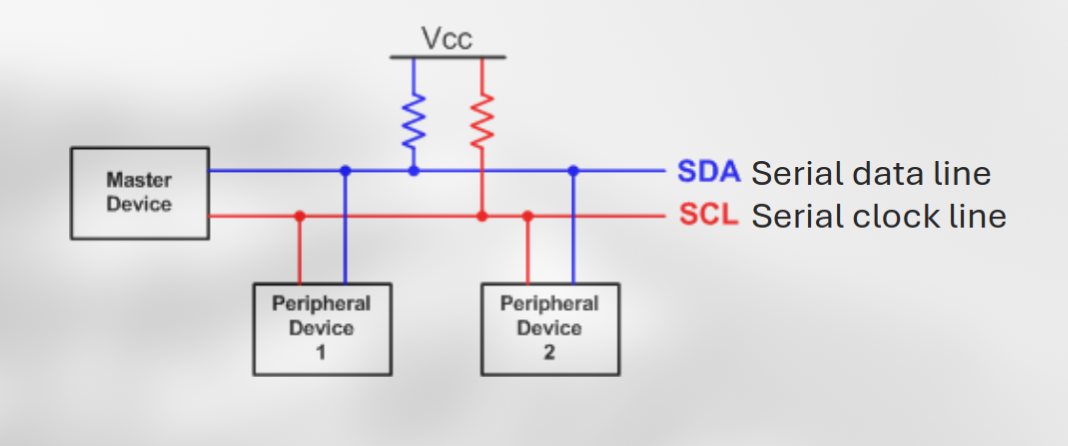
\includegraphics{images/i2c.png}
    \caption{I2C}
    \label{fig:i2c}
\end{figure}

Normal digital logic outputs are connected to push-pull drivers.
I2C signals are connected to open-drain drivers.
They cannot pull up for a logic high. Instead, a pull-up
resistor is responsible for keeping each signal high unless
it is pulled low by any I2C driver.

While SPI has faster speed and supports full
duplex, I2C is simpler and adding a new
slave is easy. We prefer I2C when it's
convenient to connect multiple devices
using only two wires, and when speed is
not critical.

I2C's slower speed is due partly
to its open-drain design, which must
wait for the line to be pulled high by
the pull-up resistors for logic high,
partly by bus capacitance, and partly
by the length of the network.
I2C has multiple modes that allow for
faster communication:
\begin{itemize}
    \item Standard mode: 0-100kb/s
    \item Fast mode: 100-400kb/s
    \item Fast mode plus: 400-1000kb/s
    \item High speed mode: 1000kb/s-3.4mbit/s
\end{itemize}
The effective data rate is less than half of the
clock rate due to addressing, acknowledgements etc.

Despite (or perhaps because of) its physical
simplicity, the I2C protocol is more complex
than SPI. I2C does not have slave select lines;
it uses either 7-bit or less commonly 10-bit
slave addressing. An I2C device starts a transaction with a START (S) bit.
It then sends a 7 or 10-bit address, followed
by a 1-bit intent. 0 for write, 1 for read.
It listens for an ACK/NACK sent by the receiver,
and then sends a STOP (P) bit.
The ACK is a logic low, and NACK is logic
high. If no device on the I2C bus will
respond to the particular address that
was sent, then nothing will acknowledge.
If nothing acknowledges, there is nothing
to pull the line low. This indicates
failure.
\marginnote{START and STOP bits
    are the only times that
    SDA changes when SCL
    is held high.}
Both addresses and data are sent
most-significant-bit first.
The I2C protocol makes no definitions
for the contents of the data fields.

When a master device writes a command and single data byte to a slave device, it looks
like Figure \ref{fig:i2cwritesingle}
\begin{figure}
    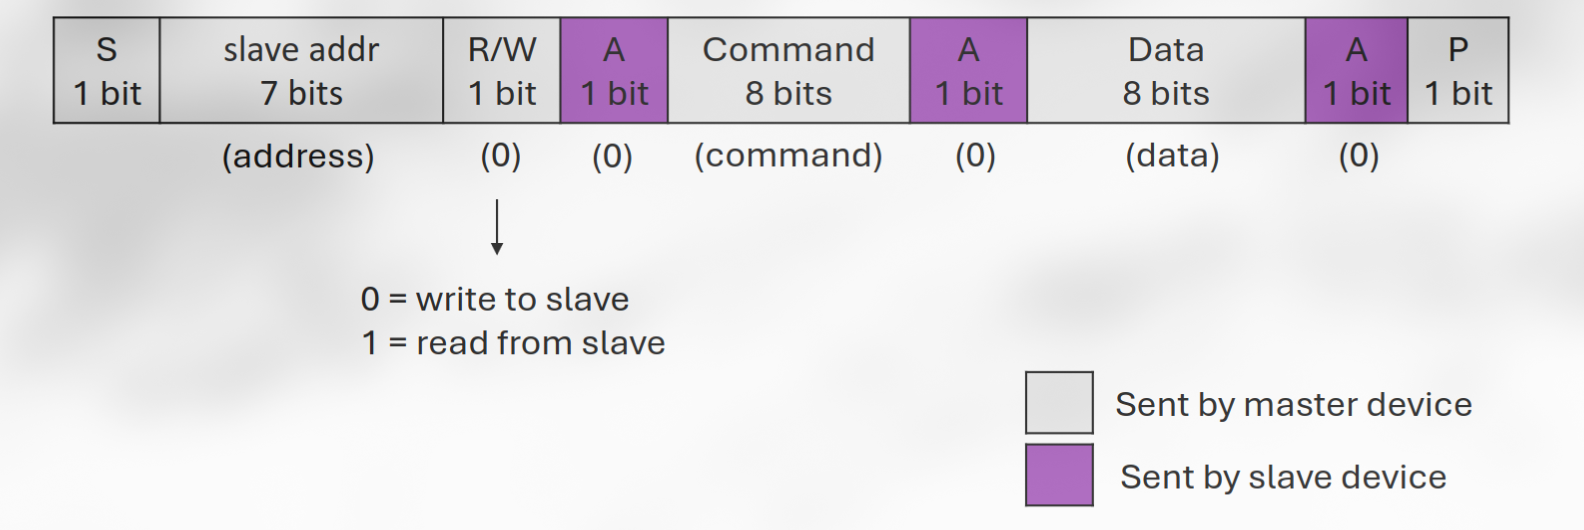
\includegraphics{images/i2cwritesingle.png}
    \caption{I2C Command Write}
    \label{fig:i2cwritesingle}
\end{figure}

When a master device reads two data bytes
from a slave device, it looks
like Figure \ref{fig:i2creaddouble}.
\begin{figure}
    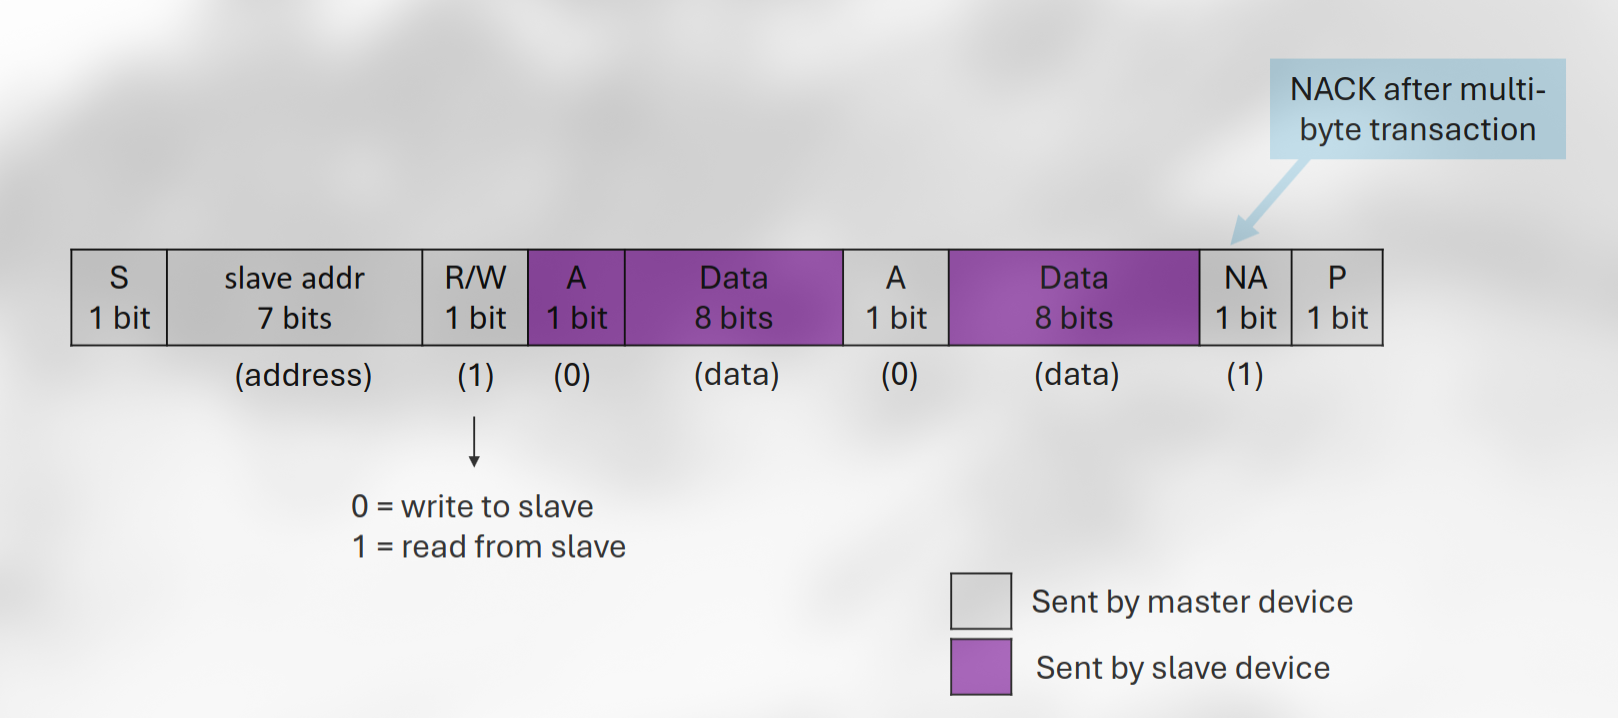
\includegraphics{images/i2creaddouble.png}
    \caption{I2C Double Read}
    \label{fig:i2creaddouble}
\end{figure}

Both the data and clock lines of an I2C bus are open-drain.
When clock stretching is enabled,
any device on the I2C bus can
lengthen the low time of a clock.
The master drives the clock, but a slave device
may not be able to keep up.
Any slave device may lengthen the clock only
after the ACK bit and before the MSB of
the next byte.